\documentclass[../main]{subfiles}
\begin{document}
% \setcounter{section}{0}
\section{基本}
%------------------------------------------------------------
\begin{figure}[H]
    \begin{minipage}{.33\textwidth}
        \centering
        \begin{equation*}
            y = ax
        \end{equation*}
        ($a$は比例定数)
    \end{minipage}
    \begin{minipage}{.33\textwidth}
        \centering
        $a>0$
        \fbox{
        \begin{tikzpicture}[scale=0.4,domain=-3:3]
            \draw[->] (-3.1,0) -- (3.1,0) node[right] {$x$};
            \draw[->] (0,-3.1) -- (0,3.1) node[above] {$y$};
            \draw[variable=\x,blue] plot({\x},{\x});
        \end{tikzpicture}}
    \end{minipage}
    \begin{minipage}{.33\textwidth}
        \centering
        $a<0$
        \fbox{\begin{tikzpicture}[scale=0.4,domain=-3:3]
            \draw[->] (-3.1,0) -- (3.1,0) node[right] {$x$};
            \draw[->] (0,-3.1) -- (0,3.1) node[above] {$y$};
            \draw[variable=\x,blue] plot({\x},{-\x});
        \end{tikzpicture}}
    \end{minipage}
    \end{figure}
%------------------------------------------------------------
\begin{figure}[H]
    \begin{minipage}{.33\textwidth}
        \centering
        \begin{equation*}
            y = \frac{a}{x}
        \end{equation*}
        ($a$は比例定数)
    \end{minipage}
    \begin{minipage}{.33\textwidth}
        \centering
        $a>0$
        \fbox{
        \begin{tikzpicture}[scale=0.4,domain=-3:3]
            \draw[->] (-3.1,0) -- (3.1,0) node[right] {$x$};
            \draw[->] (0,-3.1) -- (0,3.1) node[above] {$y$};
            \draw[domain=-3:-0.35,variable=\x,blue] plot({\x},{1/\x});
            \draw[domain=0.35:3,variable=\x,blue] plot({\x},{1/\x});
        \end{tikzpicture}}
    \end{minipage}
    \begin{minipage}{.33\textwidth}
        \centering
        $a<0$
        \fbox{\begin{tikzpicture}[scale=0.4,domain=-3:3]
            \draw[->] (-3.1,0) -- (3.1,0) node[right] {$x$};
            \draw[->] (0,-3.1) -- (0,3.1) node[above] {$y$};
            \draw[domain=-3:-0.35,variable=\x,blue] plot({\x},{-1/\x});
            \draw[domain=0.35:3,variable=\x,blue] plot({\x},{-1/\x});
        \end{tikzpicture}}
    \end{minipage}
    \end{figure}
%------------------------------------------------------------
\begin{figure}[H]
    \begin{minipage}{.33\textwidth}
        \centering
        \begin{equation*}
            y = ax+b
        \end{equation*}
        ($a$は比例定数)
    \end{minipage}
    \begin{minipage}{.33\textwidth}
        \centering
        $a>0$
        \fbox{
        \begin{tikzpicture}[scale=0.4,domain=-3:3]
            \draw[->] (-3.1,0) -- (3.1,0) node[right] {$x$};
            \draw[->] (0,-3.1) -- (0,3.1) node[above] {$y$};
            \draw[variable=\x,blue] plot({\x},{\x+1});
        \end{tikzpicture}}
    \end{minipage}
    \begin{minipage}{.33\textwidth}
        \centering
        $a<0$
        \fbox{\begin{tikzpicture}[scale=0.4,domain=-3:3]
            \draw[->] (-3.1,0) -- (3.1,0) node[right] {$x$};
            \draw[->] (0,-3.1) -- (0,3.1) node[above] {$y$};
            \draw[variable=\x,blue] plot({\x},{-\x+1});
        \end{tikzpicture}}
    \end{minipage}
    \end{figure}
%------------------------------------------------------------
\begin{figure}[H]
    \begin{minipage}{.33\textwidth}
        \centering
        \begin{equation*}
            y = ax^2
        \end{equation*}
        ($a$は比例定数)
    \end{minipage}
    \begin{minipage}{.33\textwidth}
        \centering
        $y=ax^2$
        \fbox{
        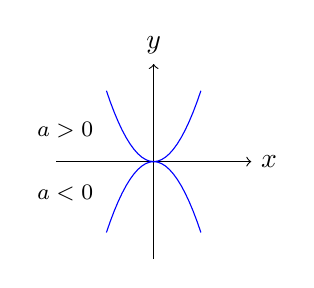
\begin{tikzpicture}[scale=0.4,domain=-1.5:1.5]
            \draw[->] (-3.1,0) -- (3.1,0) node[right] {$x$};
            \draw[->] (0,-3.1) -- (0,3.1) node[above] {$y$};
            \draw[variable=\x,blue] plot({\x},{\x*\x});
            \draw[variable=\x,blue] plot({\x},{(-1)*\x*\x});
            \path (-4,1) node[right] {\footnotesize$a>0$};
            \path (-4,-1) node[right] {\footnotesize$a<0$};
        \end{tikzpicture}}
    \end{minipage}
    \begin{minipage}{.33\textwidth}
        \centering
        $y=a(x-p)^2+q$
        \fbox{\begin{tikzpicture}[scale=0.4,domain=-0.5:2.5]
            \draw[->] (-3.1,0) -- (3.1,0) node[right] {$x$};
            \draw[->] (0,-3.1) -- (0,3.1) node[above] {$y$};
            \draw[variable=\x,blue] plot({\x},{(\x-1)^2+1});
            \path (3,0) coordinate(x);
            \path (0,3) coordinate(y);
            \path (1,1) coordinate(p);
            \path (0,0) coordinate(o);
            \draw[dashed] ($(o)!(p)!(x)$) node[below]{$p$} -- (p);
            \draw[dashed] ($(o)!(p)!(y)$) node[left]{$q$} -- (p);
        \end{tikzpicture}}
    \end{minipage}
    \end{figure}
%------------------------------------------------------------
\begin{figure}[H]
    \begin{minipage}{.33\textwidth}
        \centering
        $y=\frac{1}{x^2}$
        \fbox{
        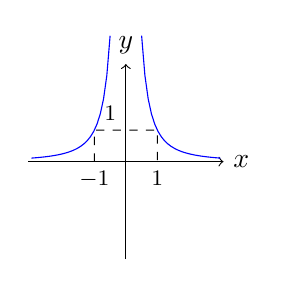
\begin{tikzpicture}[scale=0.4,domain=-3:3]
            \draw[->] (-3.1,0) -- (3.1,0) node[right] {$x$};
            \draw[->] (0,-3.1) -- (0,3.1) node[above] {$y$};
            \draw[domain=-3:-0.5,variable=\x,blue] plot({\x},{1/(\x*\x)});
            \draw[domain=0.5:3,variable=\x,blue] plot({\x},{1/(\x*\x)});
            % \path (0,0) coordinate (o) node[below right]{\footnotesize$O$};
            \path (0,1) coordinate (y1) node[above left]{\footnotesize$1$};
            \path (1,0) coordinate (x1) node[below]{\footnotesize$1$};
            \path (-1,0) coordinate (x2) node[below]{\footnotesize$-1$};
            \draw[thin,dashed] (x2) -- (-1,1) -- (1,1) -- (x1);
        \end{tikzpicture}}
    \end{minipage}
    \begin{minipage}{.33\textwidth}
        \centering
        $y=x^3$
        \fbox{
        \begin{tikzpicture}[scale=0.4,domain=-1.5:1.5]
            \draw[->] (-3.1,0) -- (3.1,0) node[right] {$x$};
            \draw[->] (0,-3.1) -- (0,3.1) node[above] {$y$};
            \draw[variable=\x,blue] plot({\x},{\x*\x*\x});
            \path (0,1) coordinate (y1) node[above left]{\footnotesize$1$};
            \path (0,-1) coordinate (y2) node[right]{\footnotesize$-1$};
            \path (1,0) coordinate (x1) node[below]{\footnotesize$1$};
            \path (-1,0) coordinate (x2) node[above]{\footnotesize$-1$};
            \draw[thin,dashed] (y2) -- (-1,-1) -- (x2);
            \draw[thin,dashed] (y1) -- (1,1) -- (x1);
        \end{tikzpicture}}
    \end{minipage}
    \begin{minipage}{.33\textwidth}
        \centering
        $y=x^4$
        \fbox{\begin{tikzpicture}[scale=0.4,domain=-1.5:1.5]
            \draw[->] (-3.1,0) -- (3.1,0) node[right] {$x$};
            \draw[->] (0,-3.1) -- (0,3.1) node[above] {$y$};
            \draw[variable=\x,blue] plot({\x},{\x*\x*\x*\x});
            \path (0,1) coordinate (y1) node[above left]{\footnotesize$1$};
            \path (1,0) coordinate (x1) node[below]{\footnotesize$1$};
            \path (-1,0) coordinate (x2) node[below]{\footnotesize$-1$};
            \draw[thin,dashed] (x2) -- (-1,1) -- (1,1) -- (x1);
        \end{tikzpicture}}
    \end{minipage}
    \end{figure}
%------------------------------------------------------------
\begin{minipage}{.4\textwidth}
    \begin{tikzpicture}[scale=1]
        \coordinate [label=left:{A}] (A) at (0,0);
        \coordinate [label=right:{B}] (B) at (5,3);
        \coordinate [label=right:{C}] (C) at (5,0);
        \draw (A) -- (B) node [midway,above] {c} -- (C) node [midway,right]{a} -- (A) node [midway,below] {b} -- cycle;
        % \draw ($(C)!5pt!(A)$) |- ($(C)!5pt!-90:(A)$);
        % \draw pic["$\theta$", draw=black, -, very thick, angle eccentricity=1.2, angle radius=1cm] {angle=C--A--B};
        % \tkzMarkRightAngle[fill=lightgray](A,C,B)
        \tkzMarkRightAngle(A,C,B)
        \tkzMarkAngle(C,A,B)
        \tkzFillAngle[fill=red,size=1,opacity=.5](C,A,B)
        \tkzLabelAngle[pos=1.2](C,A,B){$\theta$}
    \end{tikzpicture}
\end{minipage}
%------------------------------------------------------------
\begin{minipage}[c]{.4\textwidth}
    \begin{tikzpicture}
        \draw[->] (-1,0) -- (3,0) node(xaxis)[right] {$x$};
        \draw[->] (0,-1) -- (0,3) node(yaxis)[above] {$y$};
        \draw (0:2) arc [start angle=0, delta angle=100, radius=2];
        \path (0,0) coordinate (O) node[below right] {$O$};
        \path (0:2) coordinate (X) node[below] {$1$};
        \path (90:2) coordinate (Y) node[above left] {$1$};
        \fill (40:2) circle (2pt) coordinate (A) node[right=0.5em] {$(x,y)$};
        \draw (O) -- ($(O)!1.5!(A)$);
        \tkzMarkAngle[size=0.5](X,O,A);
        \tkzLabelAngle[pos=0.7](X,O,A){$\theta$};
    \end{tikzpicture}
    \end{minipage}
    \begin{minipage}[l]{.4\textwidth}
        \begin{gather*}
            x = \cos{\theta} \qquad y = \sin{\theta} \\
            \text{傾き} = \frac{y}{x} = \frac{\sin{\theta}}{\cos{\theta}} = \tan{\theta}
        \end{gather*}
    \end{minipage}
%------------------------------------------------------------
\begin{minipage}{.4\textwidth}
    \begin{tikzpicture}[scale=1]
        \path (0,0) coordinate (A) node[left] {A};
        \path (5,0) coordinate (B) node[right] {B};
        \path (3,4) coordinate (C) node[above] {C};
        \draw (A) -- (B) -- (C) node[midway,right]{a} -- cycle node[midway,left]{b};
        \path ($(A)!(C)!(B)$) coordinate (D);
        \draw (C) -- (D);
        \tkzMarkRightAngle(A,D,C);
        \tkzMarkAngle[size=0.5](D,A,C);
        \draw [red,bend right,distance=1cm,dashed] (C) to node[fill=white, inner sep=0.1cm, rectangle] {\small$b\sin{A}$} (D);
        \draw [red,bend left,distance=1cm,dashed] (A) to node[fill=white, inner sep=0.1cm, rectangle] {\small$b\cos{A}$} (D);
        \draw [red,bend left,distance=1cm,dashed] (D) to node[fill=white, inner sep=0.1cm, rectangle] {\small$c-b\cos{A}$} (B);
        \draw [bend right,distance=1cm, dashed] (A) to node[fill=white, inner sep=0.1cm, rectangle] {$c$} (B);

    \end{tikzpicture}
\end{minipage}
%------------------------------------------------------------
\begin{minipage}{.4\textwidth}
    \begin{tikzpicture}
        \path (0,0) coordinate (b) node[below] {$b$};
        \path (3,0) coordinate (c) node[below] {$c$};
        \path (3,3) coordinate (a) node[above] {$a$};
        \draw ($(c)!1.2!(b)$) -- ($(b)!1.5!(c)$);
        \draw (b) -- (a) node[midway,above]{1} -- (c);
        \path (20:4.5) coordinate (D);
        \path ($(b)!(a)!(D)$) coordinate (d) node[below right] {$d$};
        \draw (b) -- (D);
        \draw (a) -- (d);
        \path[name path=ac] (a) -- (c);
        \path[name path=bd] (b) -- (d);
        \path[name intersections={of=ac and bd, by=g}];
        \node[below right] at (g) {$g$};
        \tkzMarkAngle[size=.7](g,a,d);
        \tkzLabelAngle[pos=1.2](g,a,d){$A$};
        \tkzMarkRightAngle(b,c,a);
        \tkzMarkRightAngle(g,d,a);
        \tkzMarkAngle[size=.7](c,b,d);
        \tkzLabelAngle[pos=1.2](c,b,d){$A$};
        \tkzMarkAngle[size=.7](d,b,a);
        \tkzMarkAngle[size=.75](d,b,a);
        \tkzLabelAngle[pos=1.2](d,b,a){$B$};
    \end{tikzpicture}
\end{minipage}
\begin{minipage}{.4\textwidth}
    \begin{tikzpicture}
        \path (0,0) coordinate (b) node[below] {$b$};
        \path (3,0) coordinate (c) node[below] {$c$};
        \path (3,3) coordinate (a) node[above] {$a$};
        \draw ($(c)!1.2!(b)$) -- ($(b)!1.5!(c)$);
        \draw (b) -- (a) node[midway,above]{1} -- (c);
        \path (20:4.5) coordinate (D);
        \path ($(b)!(a)!(D)$) coordinate (d) node[below right] {$d$};
        \draw (b) -- (D);
        \draw (a) -- (d);
        \path ($(a)!(d)!(c)$) coordinate (f) node[left] {$f$};
        \draw (d) -- (f);
        \path ($(b)!(d)!(c)$) coordinate (e) node[below] {$e$};
        \draw (d) -- (e);
        \tkzMarkAngle[size=.7](c,a,d);
        \tkzLabelAngle[pos=1.2](c,a,d){$A$};
        \tkzMarkAngle[size=.7](c,b,d);
        \tkzLabelAngle[pos=1.2](c,b,d){$A$};
        \tkzMarkAngle[size=.7](d,b,a);
        \tkzMarkAngle[size=.75](d,b,a);
        \tkzLabelAngle[pos=1.2](d,b,a){$B$};
    \end{tikzpicture}
\end{minipage}
%------------------------------------------------------------
%------------------------------------------------------------
%------------------------------------------------------------
%------------------------------------------------------------
%------------------------------------------------------------
%------------------------------------------------------------
%------------------------------------------------------------
%------------------------------------------------------------
%------------------------------------------------------------
%------------------------------------------------------------
%------------------------------------------------------------
\end{document}